\hypertarget{nat-traversal}{%
\chapter{NAT Traversal}\label{nat-traversal}}

\begin{figure}
\centering
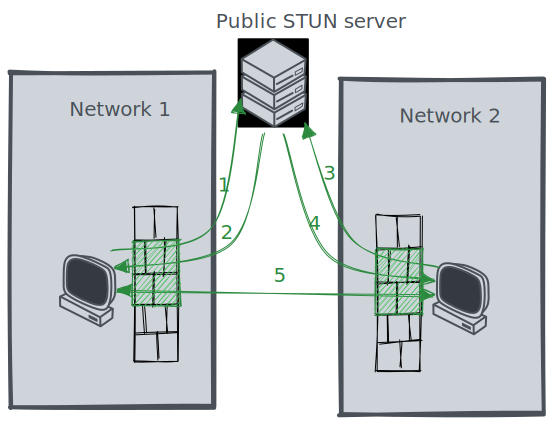
\includegraphics[width=\textwidth,height=0.66\textheight]{presentation/../figures/nat-traversal.png}
\caption{``NAT traversal via STUN''\label{nat-traversal}}
\end{figure}

\begin{itemize}
\tightlist
\item
  Session Traversal Utilities for NAT (STUN)

  \begin{itemize}
  \tightlist
  \item
    Parties connect to a public STUN server (can be another party)
  \item
    The server reports the IPs it ``sees'' the parties at
  \item
    User Datagram Protocol (UDP) hole punching

    \begin{itemize}
    \tightlist
    \item
      Reverse channel for the STUN server to talk back to a party
    \item
      Appropriated by the other parties for their own traffic
    \end{itemize}
  \end{itemize}
\end{itemize}
